% !TEX program = xelatex
\documentclass[a4paper]{article}
\usepackage{amsthm}
\usepackage{amssymb}
\usepackage{bm}
\usepackage{mathtools}
\usepackage[x11names]{xcolor}
\usepackage{xparse}
\usepackage{fontspec}
\usepackage{unicode-math}
\setromanfont[Ligatures={Common,Rare}]{DovesType-Regular.otf}
\setsansfont{Andika}
\setmathfont{Asana Math}[Scale=1]
\newfontfamily\TrajanP[Scale=1.0]{TRAJANPRO-REGULAR.OTF}
% \newfontfamily\TrajanP[Scale=1.0]{Tork}

% \usepackage{pstricks}
\usepackage{varwidth}
\usepackage{siunitx}
\usepackage{graphicx}
\usepackage[margin=1.5cm,top=1.5cm]{geometry}
\usepackage[most]{tcolorbox}
\usepackage{pgfplots}
\pgfplotsset{compat=newest}
\tcbuselibrary{skins,xparse,poster,breakable}
% \usetikzlibrary{fadings}
\usetikzlibrary{calc,math, plotmarks, shapes, shapes.geometric, positioning, angles, intersections, quotes, through, patterns, turtle, arrows.meta}
\usetikzlibrary{decorations.markings,backgrounds}
% \usepackage{etoolbox}
\usepackage{tkz-euclide}
\usetkzobj{all}
% \usepackage{xlop}
% \newcommand\hole[2]{#1}  % for use with xlop
\pagenumbering{gobble}
%%%%%%%%%%%%%%%%%%%%%%%%%%%%%%%%%%%%%%%%%%%%%%%%%%%%%%%%%
\newcommand\markangle[9]{% origin X Y radius radiusmark mark colour opacity
%  % fill red circle offset-from-centre
  \begin{scope}
    \path[clip] (#1) -- (#2) -- (#3);
    \fill[color=#7,fill opacity=#8,draw=black,name path global=pcircle]  % global declaration required otherwise pcircle is not seen by the `named intersections=' lines below.
    (#1) circle (#4);
  \end{scope}
  % middle calculation
  \path[name path=line one] (#1) -- (#2);
  \path[name path=line two] (#1) -- (#3);
  \path[%
  name intersections={of=line one and pcircle, by={inter one}},
  name intersections={of=line two and pcircle, by={inter two}}
  ] (inter one) -- (inter two) coordinate[pos=#9] (place);
  % put mark
  \node at ($(#1)!#5!(place)$) {\scriptsize{#6}};
}
%%%%%%%%%%%%%%%%%%%%%%%%%%%%%%%%%%%%%%%%%%%%%%%%%%%%%%%%
\newcommand\tcircle[6]{% centre coord (x,y), radius, points, radpoint, colour, edge
  \coordinate (O) at (#1,#2); % centre of the circle
  \def\radius{#3}          % radius of the circle
  \def\npts{#4}            % number of the points
  \def\radpt{#5}           % radius of the points
  \colorlet{ptcolour}{#6}  % colour of the points
  % \draw (O) circle (\radius);
  \foreach \numpoint in {1,...,\npts}{
    \fill[ptcolour] (O) ++ (360/\npts*\numpoint:\radius) coordinate (C\numpoint) circle(\radpt);
  }
}

% \newcommand{\condSoln}[2]{\ifcsdef{r@#1}{#2}{}}

% \newcommand\fadingtext[3][]{%
%    \begin{tikzfadingfrompicture}[name=fading letter]
%      \node[text=transparent!0,inner xsep=0pt,outer xsep=0pt,#1] {#3};
%    \end{tikzfadingfrompicture}%
%    \begin{tikzpicture}[baseline=(textnode.base)]
%      \node[inner sep=0pt,outer sep=0pt,#1](textnode){\phantom{#3}};
%      \shade[path fading=fading letter,#2,fit fading=false]
%      (textnode.south west) rectangle (textnode.north east);%
%    \end{tikzpicture}%
% }

\definecolor{JISpurple}{RGB}{89,72,122}
\definecolor{JISivory}{RGB}{241,234,221}
\definecolor{JIStaupe}{RGB}{183,156,154}
\definecolor{PaleGreen}{RGB}{240,255,240} % 'Honeydew'

\AddToHook{shipout/background}{%
    \put (0in,-\paperheight){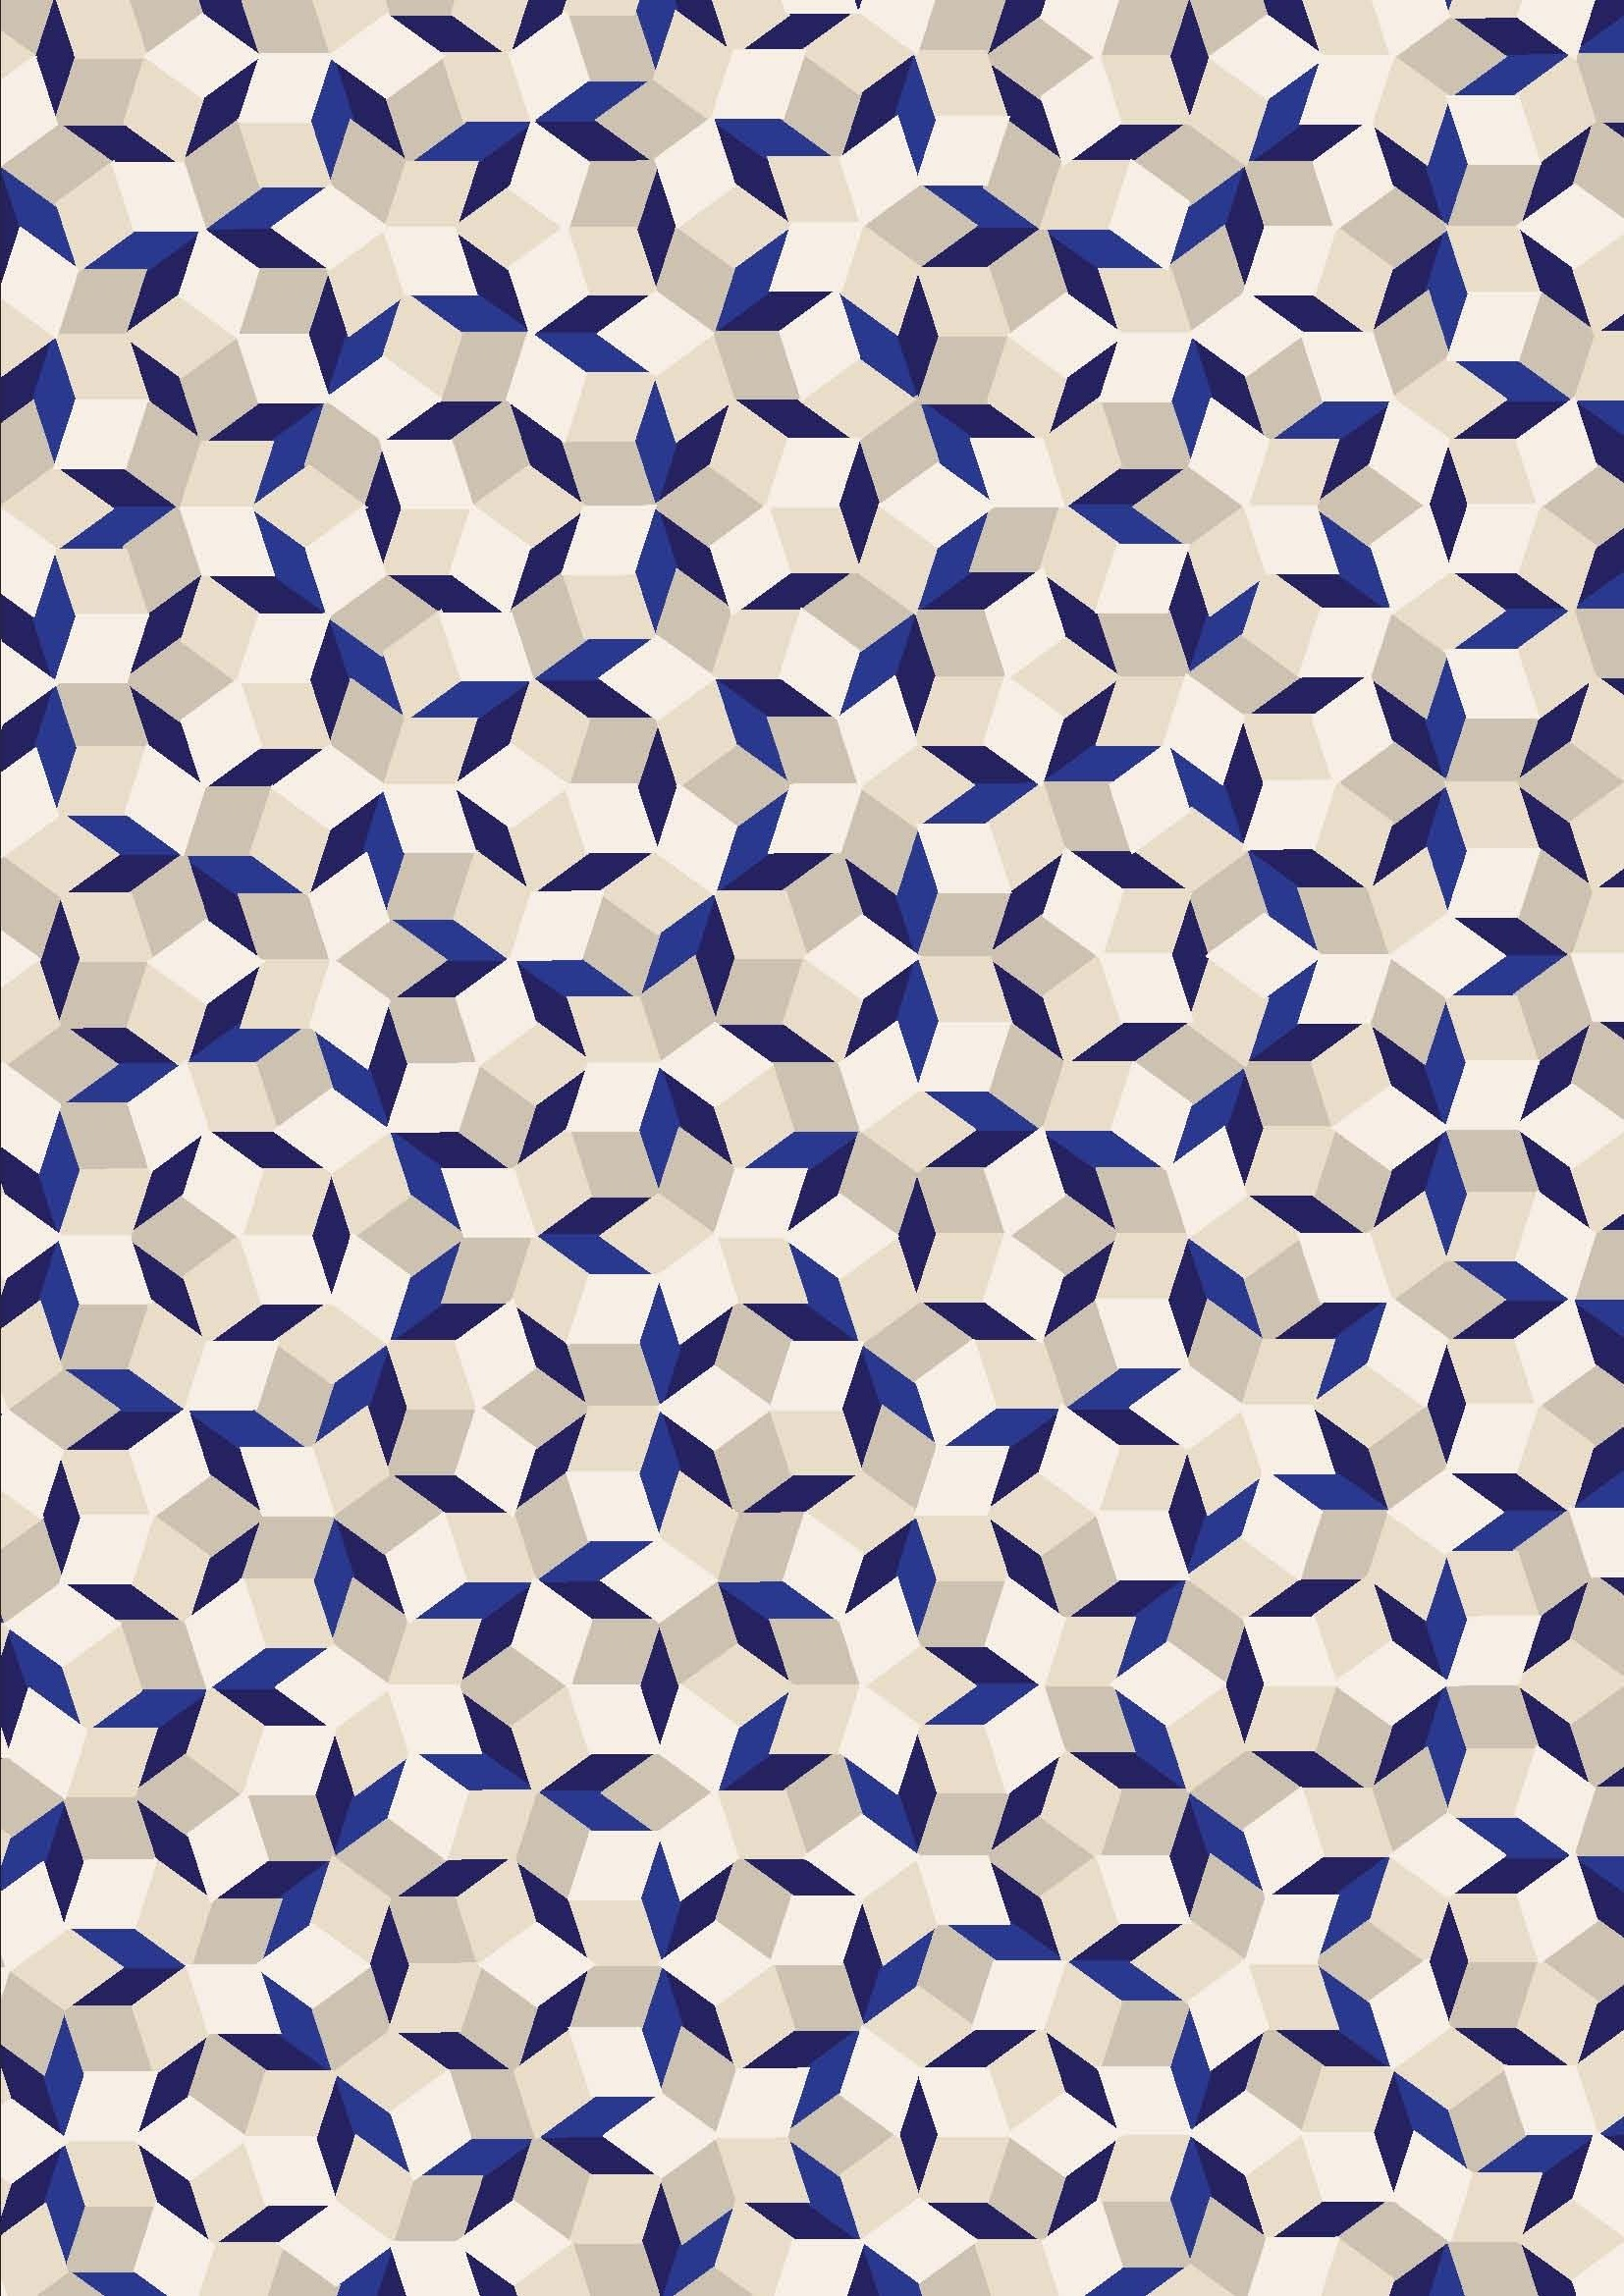
\includegraphics[width=\paperwidth,height=\paperheight]{images/penrose2r.jpg}}%
}

\newcommand\numberthis{\addtocounter{equation}{1}\tag{\theequation}}

\newtcolorbox{MyOuterBox}{%
  enhanced,
  % watermark graphics=images/santa_faces_watermark.jpg,
  % watermark opacity=0.8,
  % watermark zoom=2.0,
  breakable,
  frame style=JISpurple,
  colback=JISivory,
  colframe=JISpurple,
  title={
\includegraphics[width=0.9cm,height=0.9cm]{images/JIS Final Logo FA-02.png}\raisebox{3mm}{\Large{Maths Challenge}\hspace{24em} \Large{\bfseries\sffamily 21}}},
}

\newtcolorbox{MyInnerBox}[2][]{enhanced,%empty,
coltitle=JISpurple,colback=white,
breakable,
fonttitle=\bfseries\sffamily,
attach boxed title to top left={yshift=-1.5mm},
boxed title style={empty, size=small, top=1mm, bottom=0pt},
varwidth boxed title=0.5\linewidth,
frame code={
  \path (title.east|-frame.north) coordinate (aux);
\path[draw=JISpurple, line width=0.5mm, rounded corners,fill=white]
(frame.west) |- ([xshift=-2.5mm]title.north east) to[out=0, in=180] ([xshift=7.5mm]aux)-|(frame.east)|-(frame.south)-|cycle;
},
title={#2},#1}

\newtcolorbox{MyInnerSplitBox}[2][]{enhanced,%empty,
bicolor,sidebyside,sidebyside align=top seam,
righthand width=7.0cm,colbacklower=white,
sidebyside gap=5mm,
breakable,
coltitle=JISpurple,colback=white,
fonttitle=\bfseries\sffamily,
attach boxed title to top left={yshift=-1.5mm},
boxed title style={empty, size=small, top=1mm, bottom=0pt},
varwidth boxed title=0.5\linewidth,
frame code={
  \path (title.east|-frame.north) coordinate (aux);
\path[draw=JISpurple, line width=0.5mm, rounded corners,fill=white]
(frame.west) |- ([xshift=-2.5mm]title.north east) to[out=0, in=180] ([xshift=7.5mm]aux)-|(frame.east)|-(frame.south)-|cycle;
},
title={#2},#1}


\newtcolorbox{MySolutionBox}[1][]{%
  enhanced,
  breakable,
  frame style=JISpurple,
  colback=PaleGreen, colframe=green,
  title={\Large Solution},
  drop fuzzy shadow,
  halign=left,
  #1
}

%%%%%%%%%%%%%%%%%%%%%%%%%%%%%%%%%%%%%%%%%%%%%%%%%%
\newtoggle{SOLUTION}
%%% Uncomment the appropriate line below to show solutions %%%
\toggletrue{SOLUTION}
% \togglefalse{SOLUTION}
%%%%%%%%%%%%%%%%%%%%%%%%%%%%%%%%%%%%%%%%%%%%%%%%%


%%%%%%%%%%%%%%%%%%%%%%%%%%%%%%%%%%%%%%%%%%%%%%%%%%
%%%%%%            DOCUMENT BEGINS           %%%%%%
%%%%%%%%%%%%%%%%%%%%%%%%%%%%%%%%%%%%%%%%%%%%%%%%%%
\begin{document}


  \begin{MyOuterBox}
    \iftoggle{SOLUTION}{Here are the full, or partial solutions.
    }{
      Welcome to this week's Maths Challenge!\\
      Have a go at both questions!\\
      Drop your solution in the box in the staffroom by Tuesday.
    }
       \begin{MyInnerBox}{Year 8 and below}
     A Pattern of squares. All six coloured areas are equal. What fraction is shaded?\par\medskip
     \begin{tikzpicture}[scale=1]
       \draw[thick] (0,0) coordinate (A) -- (3,0) coordinate (B) -- (3,3) coordinate (C) -- (0,3) coordinate (D) -- cycle;
       \draw[thick,fill=SeaGreen2] (A) -- (0,1) -- (1,1) -- (1,0) -- cycle;
       \draw[thick,fill=RoyalBlue2] (2,0) -- (B) -- (3,1) -- (2,1) -- cycle;
       \draw[thick,fill=Yellow2] (2,2) -- (3,2) -- (C) -- (2,3) -- cycle;
       \draw[thick,fill=PaleTurquoise1] (0,2) -- (1,2) -- (1,3) -- (D) -- cycle;
       \draw[thick,fill=Orange1] (0.5,1.5) -- (1.5,0.5) -- (2.5,1.5) -- (1.5,2.5) -- cycle;
       \draw[thick,fill=Tomato1] ({1-((sqrt(2)-1)/2)},1.5) -- (1.5,{1-((sqrt(2)-1)/2}) -- ({2+((sqrt(2)-1)/2)},1.5) -- (1.5,{2+((sqrt(2)-1)/2)}) -- cycle;
       \iftoggle{SOLUTION}{
         \node[above] at (D) {\(1\)};
         \draw[blue,-{Triangle[width=10pt,length=7pt]}, line width=4pt] (3.1,1.5) -- (3.8,1.5);
         \draw[thick,<-] ([shift=(30:0.3cm)]1.5,1.5) arc (30:300:0.3cm);
     }{}
     \end{tikzpicture}%
     \iftoggle{SOLUTION}{
     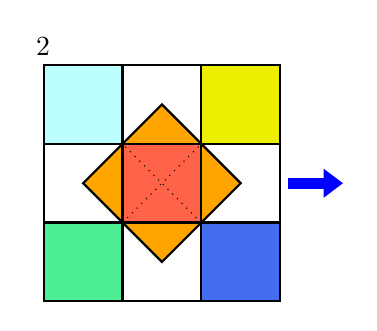
\begin{tikzpicture}[scale=1]
       \draw[thick] (0,0) coordinate (A) -- (3,0) coordinate (B) -- (3,3) coordinate (C) -- (0,3) coordinate (D) -- cycle;
       \draw[thick,fill=SeaGreen2] (A) -- (0,1) -- (1,1) -- (1,0) -- cycle;
       \draw[thick,fill=RoyalBlue2] (2,0) -- (B) -- (3,1) -- (2,1) -- cycle;
       \draw[thick,fill=Yellow2] (2,2) -- (3,2) -- (C) -- (2,3) -- cycle;
       \draw[thick,fill=PaleTurquoise1] (0,2) -- (1,2) -- (1,3) -- (D) -- cycle;
       \draw[thick,fill=Orange1] (0.5,1.5) -- (1.5,0.5) -- (2.5,1.5) -- (1.5,2.5) -- cycle;
       \draw[thick,fill=Tomato1] (1,1) -- (2,1) -- (2,2) -- (1,2) -- cycle;
       \draw[dotted] (1,1) -- (2,2) (2,1) -- (1,2);
         \node[above] at (D) {\(2\)};
         \draw[blue,-{Triangle[width=10pt,length=7pt]}, line width=4pt] (3.1,1.5) -- (3.8,1.5);
     \end{tikzpicture}%
     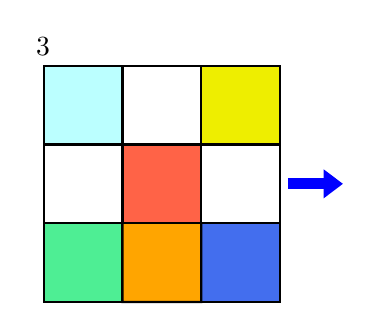
\begin{tikzpicture}[scale=1]
       \draw[thick] (0,0) coordinate (A) -- (3,0) coordinate (B) -- (3,3) coordinate (C) -- (0,3) coordinate (D) -- cycle;
       \draw[thick,fill=SeaGreen2] (A) -- (0,1) -- (1,1) -- (1,0) -- cycle;
       \draw[thick,fill=RoyalBlue2] (2,0) -- (B) -- (3,1) -- (2,1) -- cycle;
       \draw[thick,fill=Yellow2] (2,2) -- (3,2) -- (C) -- (2,3) -- cycle;
       \draw[thick,fill=PaleTurquoise1] (0,2) -- (1,2) -- (1,3) -- (D) -- cycle;
       \draw[thick,fill=Orange1] (1,0) -- (2,0) -- (2,1) -- (1,2) -- cycle;
       \draw[thick,fill=Tomato1] (1,1) -- (2,1) -- (2,2) -- (1,2) -- cycle;
         \node[above] at (D) {\(3\)};
         \draw[blue,-{Triangle[width=10pt,length=7pt]}, line width=4pt] (3.1,1.5) -- (3.8,1.5);
     \end{tikzpicture}%
     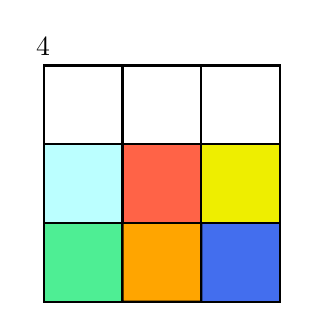
\begin{tikzpicture}[scale=1]
       \draw[thick] (0,0) coordinate (A) -- (3,0) coordinate (B) -- (3,3) coordinate (C) -- (0,3) coordinate (D) -- cycle;
       \draw[thick,fill=SeaGreen2] (A) -- (0,1) -- (1,1) -- (1,0) -- cycle;
       \draw[thick,fill=RoyalBlue2] (2,0) -- (B) -- (3,1) -- (2,1) -- cycle;
       \draw[thick,fill=Yellow2] (2,1) -- (3,1) -- (3,2) -- (2,2) -- cycle;
       \draw[thick,fill=PaleTurquoise1] (0,1) -- (1,1) -- (1,2) -- (0,2) -- cycle;
       \draw[thick,fill=Orange1] (1,0) -- (2,0) -- (2,1) -- (1,2) -- cycle;
       \draw[thick,fill=Tomato1] (1,1) -- (2,1) -- (2,2) -- (1,2) -- cycle;
       \draw[thick] (1,3) -- (1,2) (2,3) -- (2,2);
         \node[above] at (D) {\(4\)};
     \end{tikzpicture}%
     }{}
      \iftoggle{SOLUTION}{%conditional output begin
      \begin{MySolutionBox}
        See the diagrams above.\par
        Since the red square has the same area as the orange area, we can rotate the red square as shown in the second diagram, and rearrange the orange area such that the orange triangles fit exactly into the red triangles indicated by the dotted diagonal lines.\par
        We have shown that the width and height of the unshaded areas are the same as the width and height of the shaded squares.\par
        So we can fill the bottom, middle square exactly with the orange triangles (Diagram 3).\par
        Moving the cyan and yellow squares down (Diagram 4), we see that \(\frac{2}{3}\) of the diagram is shaded.\par
      \end{MySolutionBox}
    }{}%conditional output end
    \end{MyInnerBox}


    \vspace{0.4cm}
    \begin{MyInnerSplitBox}{Year 9 and above}
  Find the shaded area.\par
  \iftoggle{SOLUTION}{%conditional output begin
    \begin{MySolutionBox}
      There doesn't seem to be enough information given to be able to solve this! Yet\dots\par
      Shaded area \(A\)= area of the quadrant - area of the circle.
      \begin{align*}
        A &= \frac{\pi R^{2}}{4} - \pi r^{2}\\
        \shortintertext{In \(\bigtriangleup BDF\), we can apply Pythagoras' Thm.:}
        R^{2} &= (2r)^{2} + 12^{2}\\
        r^{2} &= \frac{R^{2}-144}{4}\\
        \shortintertext{Substituting:}
        A &= \frac{\pi R^{2}}{4} - \pi \frac{R^{2}-144}{4}\\
        A &= \frac{\pi R^{2}}{4} - \frac{\pi R^{2}}{4} + 36\pi\\
        A &= 36\pi \approx \SI{113.097}{\square\cm}
      \end{align*}
      The unknowns just vanish, isn't that marvellous?! Notice the radius of the shaded quadrant is not fixed, as long as the chord tangent to the inner circle is \(\SI{12}{\cm}\), \(R\) and \(r\) change so that the shaded area remains \(36\pi\).\par
    \end{MySolutionBox}
  }{}%conditional output end
  \tcblower
  \begin{tikzpicture}[scale=1]
    \draw[black,fill=Plum2] (6,1) coordinate (C) -- (0,1) coordinate (B) -- (0,7) coordinate (A) to[bend left=45] (C);
    \draw[black,fill=white] (3,3) coordinate (E) circle (2);
    \draw[black] (0,5) coordinate (F) -- ({sqrt(20)},5) coordinate (D) node[midway,above] {\(\SI{12}{\cm}\)};
    \tkzMarkRightAngle[draw=black,size=0.15](B,F,D);
    \iftoggle{SOLUTION}{
      \draw[gray] (B) -- (D) node[midway,above,rotate=45,black] {\(R\)};
      \draw[gray] (E) -- (3,1) node[midway,right,black] {\(r\)};
      \draw[gray,dashed,Stealth-Stealth] (-0.6,1) -- (-0.6,5) node[black,midway,inner sep=0,fill=white] {\(2r\)};
      % \draw[gray,dashed,Stealth-Stealth] (-0.6,5) -- (-0.6,7) node[black,midway,inner sep=0,fill=white] {\(R-2r\)};
      \node[below left] at (B) {\(B\)};
      \node[above right] at (D) {\(D\)};
      \node[left] at (F) {\(F\)};
    }{}
  \end{tikzpicture}
\end{MyInnerSplitBox}


  \end{MyOuterBox}

%%%%%%%%%%%%%%%%%%%%%%%%%%%%%%%%%%%%%%%%%%%%%%%%%%
\end{document}



